\chapter{Regularized Regression: Lasso, Ridge, and Elastic Net \label{chapter:lassoridge}}

In Chapter~\ref{chapter:featureselection}, we discussed embedded feature selection methods. These methods incorporate feature selection into the process of model training. Decision trees and tree ensembles (boosted trees, random forests) naturally perform feature selection in the process of model training, and will simply ignore irrelevant features. 

Regression methods, however, have a harder time. When people began to want to apply regression methods to supervised learning problems with large numbers of predictors -- particularly when the number of predictors was greater than the number of samples, or when the predictors were highly correlated -- they faced serious problems of overfitting and model instability. This led to the development of \textbf{regularized regression} (a.k.a. \textbf{penalized regression}) methods, which introduce penalty terms into the objective functions being optimized in the model fitting process to try to control the size of the coefficients assigned to various predictors and/or set some of them to zero. The goal of these methods is to allow researchers to stick with the machinery of regression models while reducing the possibility of overfitting. 

%%%%%%%%%%%%%%%%%%%%%%%%%%%%%%%%%%%%%%%%%%%%%%%%%%%%%%%%%%%%%%%%%%%%%%%%%%%%%%%%

\section{Linear Regression}

Linear regression (Chapters~\ref{chapter:regression}, \ref{chapter:linreg}, and \ref{chapter:glms}) uses the mean-squared loss:
$$ \text{loss} = \sum_{i=1}^N (y^{(i)} - \beta^T x^{(i)})^2 $$
where $\beta^T x^{(i)} = \beta_0 + \beta_1 x_1^{(i)} + \dots + \beta_p x_p^{(i)}$ is the model's prediction for the $i$th training example. To minimize the loss, we adjust the $\beta$s to make the model's predictions close to the true $y^{(i)}$ values. This is equivalent to maximizing the likelihood (see Section~\ref{section:mleglms}). 

%%%%%%%%%%%%%%%%%%%%%%%%%%%%%%%%%%%%%%%%%%%%%%%%%%%%%%%%%%%%%%%%%%%%%%%%%%%%%%%%

\section{Logistic Regression}

Logistic regression (Chapters~\ref{chapter:classification}, \ref{chapter:logreg}, and \ref{chapter:glms}) uses the negative binomial log-likelihood as its loss (compare the expression below to the one in Chapter~\ref{chapter:glms}:
$$ \text{loss} = -\sum_{i=1}^n \left[ y^{(i)} \beta^T x^{(i)} - \log \left(1 + \exp(\beta^T x^{(i)}) \right) \right]. $$
The expression has a negative sign in front because high log-likelihood is a good thing; we want low values of the log-likelihood to correspond to high values of the loss.

%%%%%%%%%%%%%%%%%%%%%%%%%%%%%%%%%%%%%%%%%%%%%%%%%%%%%%%%%%%%%%%%%%%%%%%%%%%%%%%%

\section{Lasso, Ridge, and Elastic Net Penalties}

In situations where there is a risk of overfitting and model instability (e.g., highly correlated predictors, more predictors than training examples), one can apply a penalty term to the loss function to prevent the model coefficients from taking on unrealistically large or small values. 

\subsection{Lasso Penalty}

The \textbf{Lasso}, or \textbf{L1}, penalty is related to the sum of the absolute values of the coefficients:

$$ \text{penalty}_\text{Lasso} = \lambda \sum_{j=1}^p \vert \beta_j \vert $$

This penalty will tend to cause the model to perform feature selection, setting some of the $\beta$s to zero. The values of the others may shrink, or they may be unaffected. 

\subsection{Ridge Penalty}

The \textbf{ridge}, or \textbf{L2}, penalty is related to the sum of the squared values of the coefficients:

$$ \text{penalty}_\text{ridge} = \lambda \sum_{j=1}^p \beta_j^2 $$

This penalty will tend to shrink the values of all of the model coefficients without setting any to zero. 

\subsection{Elastic Net Penalty}

The \textbf{elastic net} penalty is just a weighted sum of the Lasso and ridge penalties:

$$ \text{penalty}_\text{EN} = \lambda \left[ \alpha \sum_{j=1}^p \vert \beta_j \vert + (1-\alpha)  \sum_{j=1}^p \beta_j^2 \right] $$

The parameter $\alpha$ governs the relative weights of the two penalties. In practice, $\lambda$ and $\alpha$ are set using cross-validation. The value of $\lambda$ is unconstrained, but $\alpha$ must lie between 0 and 1. 

\begin{question}{}
This picture, from \emph{Elements of Statistical Learning} (Figure 6.7) is a geometric picture of what happens to the coefficients under the Lasso and ridge penalties.
\begin{center}
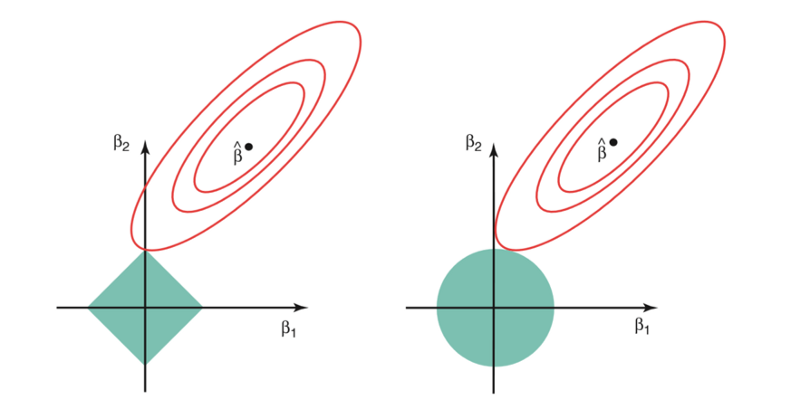
\includegraphics[width=0.8\textwidth]{img/esl-lasso-ridge-6.7.png}
\end{center}
Which picture is which? What are the red ellipses? What are the blue shapes? Do you see why Lasso is more likely than ridge to set some of the coefficients to zero?
\end{question}

%%%%%%%%%%%%%%%%%%%%%%%%%%%%%%%%%%%%%%%%%%%%%%%%%%%%%%%%%%%%%%%%%%%%%%%%%%%%%%%%

\section{Example: Predicting Blood Pressure}

Imagine we have collected blood pressure data on $10$ patients. In addition, we have information on the patients' sex, age, and obesity status. 

{\small
\begin{center}
\begin{tabular}{cccccc}
  \toprule
 & sexf & sexm & age & obesity & blood\_pressure \\ 
  \midrule
  1 & 0 & 1 & 54 & 1 & 123 \\ 
  2 & 1 & 0 & 66 & 0 & 111 \\ 
  3 & 1 & 0 & 23 & 0 & 98 \\ 
  4 & 0 & 1 & 59 & 1 & 154 \\ 
  5 & 0 & 1 & 76 & 1 & 199 \\ 
  6 & 1 & 0 & 33 & 0 & 101 \\ 
  7 & 0 & 1 & 35 & 1 & 91 \\ 
  8 & 1 & 0 & 54 & 0 & 133 \\ 
  9 & 1 & 0 & 21 & 0 & 116 \\ 
  10 & 0 & 1 & 26 & 0 & 121 \\
  \bottomrule
\end{tabular}
\end{center}
}

Note: These data are from an example in the paper ``Predictive analytics with gradient boosting in clinical medicine'', by Zhang et al, published in \emph{Annals of Translational Medicine} in 2019.

\vspace{2mm}
\begin{question}{}
Which two predictors in this model are clearly correlated?
\end{question}

We will now try many different values of $\lambda$ and $\alpha$ on these data and see what happens to the coefficients. To do this, we use the \texttt{glmnet} package in R. Here are the results:

{\small
\begin{center}
\begin{tabular}{rrrrrrr}
  \toprule
 & lambda & alpha & beta\_sexf & beta\_sexm & beta\_age & beta\_obesity \\ 
  \midrule
1 & 0.0 & 0.0 & -24.61 & -0.00 & 1.15 & -13.78 \\ 
  2 & 1.0 & 0.0 & -11.19 & 10.71 & 1.09 & -9.97 \\ 
  3 & 5.0 & 0.0 & -8.25 & 8.24 & 0.91 & -2.11 \\ 
  4 & 10.0 & 0.0 & -6.97 & 6.99 & 0.77 & 1.66 \\ 
  5 & 0.0 & 0.2 & -24.61 & -0.00 & 1.15 & -13.78 \\ 
  6 & 1.0 & 0.2 & -10.35 & 9.73 & 1.07 & -7.84 \\ 
  7 & 5.0 & 0.2 & -6.81 & 6.72 & 0.88 & 0.00 \\ 
  8 & 10.0 & 0.2 & -6.10 & 6.07 & 0.76 & 0.00 \\ 
  9 & 0.0 & 0.5 & -24.61 & -0.00 & 1.15 & -13.78 \\ 
  10 & 1.0 & 0.5 & -9.09 & 8.04 & 1.04 & -4.38 \\ 
  11 & 5.0 & 0.5 & -5.65 & 5.50 & 0.87 & 0.00 \\ 
  12 & 10.0 & 0.5 & -3.84 & 3.77 & 0.71 & 0.00 \\ 
  13 & 0.0 & 1.0 & -24.61 & -0.00 & 1.15 & -13.78 \\ 
  14 & 1.0 & 1.0 & -13.15 & 0.00 & 1.00 & 0.00 \\ 
  15 & 5.0 & 1.0 & -6.93 & 0.00 & 0.84 & 0.00 \\ 
  16 & 10.0 & 1.0 & 0.00 & 0.00 & 0.62 & 0.00 \\ 
   \bottomrule
\end{tabular}
\end{center}
}

\begin{question}{}
Which values for $\lambda$ and $\alpha$ correspond to: (a) unregularized linear regression, (b) pure Lasso, (c) pure ridge, (d) elastic net with an even combination of Lasso and ridge penalties? What happens to the values of the coefficients in each case?
\end{question}


